We connect MATLANG with arithmetic circuits as follows.

We first show that for every MATLANG expression $e$ we can associate a uniform arithmetic circuit family $\{\Phi_n^e\mid n=1,2,\ldots\}$ such that when $I$ is matrix instance of dimension $n$ (or $n\times n$), we can obtain $e(I)$ by evaluating $\Phi_n$ on $I$. \floris{The connection between the dimensions of instances etc and the ``$n$'' in the arithmetic circuits needs to be made precise. E.g., if we have $n^2$ matrices, we need more than $n$ variables...}

For a circuit $\Phi$, $\Phi[i]$ denotes its $i$-th output gate. Also, when we write $a \oplus b$ we mean 

\begin{center}
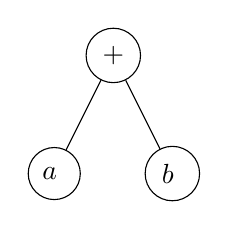
\begin{tikzpicture}[level distance=1.5cm,
  level 1/.style={sibling distance=1.5cm},
  every node/.style = {
  	shape=circle,
    draw,
    align=center,
    top color=white,
    bottom color=white
    }]
  \node {\( + \)}
    child {node { \( a \) }}
    child {node { \( b \) }};
\end{tikzpicture}
\end{center}

When we write $\bigoplus_{l=1}^n a_l$ we mean 

\begin{center}
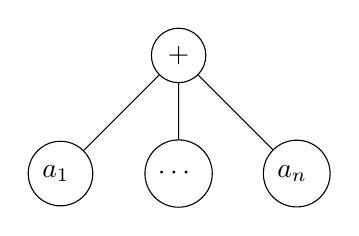
\begin{tikzpicture}[level distance=1.5cm,
  level 1/.style={sibling distance=1.5cm},
  every node/.style = {
  	shape=circle,
    draw,
    align=center,
    top color=white,
    bottom color=white
    }]
  \node {\( + \)}
    child {node { \( a_1 \) }}
    child {node { \( \cdots \) }}
    child {node { \( a_n \) }};
\end{tikzpicture}
\end{center}

Same with $\otimes$.

Let $e$ be a \langfor expression. If $e=V$ we have
\begin{itemize}
	\item When $V$ is $1\times 1$ then $\Phi^e_1$ has the one input/output gate (\textit{not necessary, covered in second item}).
	\item When $V$ is $n\times 1$ or $1\times n$ then $\Phi^e_n$ has $n$ input/output gates.
	\item When $V$ is $n\times n$ then $\Phi^e_n$ has $n^2$ input/output gates. Here, $V_{ij}=\Phi_n(V)\left[ j+n(i-1)\right]$ and $i,j=1,\ldots, n$ (entries listed row by row).
\end{itemize}

If $e=e'^T$ then $\Phi^e_n=\Phi^{e'}_n$. 

If $e=e_1 + e_2$ we have

\begin{itemize}
	\item When $e$ is $1\times 1$ then $\Phi^e_1$ is $\Phi^{e_1}_1 \oplus \Phi^{e_2}_1$.
	\item When $e$ is $n\times 1$ or $1\times n$ then $\Phi^e_n$ has $n$ output gates, where gate $k$ is $\Phi^{e_1}_n[k] \oplus \Phi^{e_2}_n[k]$.
	\item When $V$ is $n\times n$ then $\Phi^e_1$ has $n^2$ output gates, where gate $k$ is $\Phi^{e_1}_n[k] \oplus \Phi^{e_2}_n[k]$.
\end{itemize}

If $e=f(e_1, \ldots, e_k)$ we have

\begin{itemize}
	\item When $e$ is $1\times 1$ (only case necessary) then $\Phi^e_1$ is 
	
\begin{center}
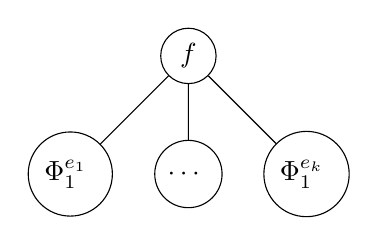
\begin{tikzpicture}[level distance=1.5cm,
  level 1/.style={sibling distance=1.5cm},
  every node/.style = {
  	shape=circle,
    draw,
    align=center,
    top color=white,
    bottom color=white
    }]
  \node {\( f \)}
    child {node { \( \Phi^{e_1}_1 \) }}
    child {node { \( \cdots \) }}
    child {node { \( \Phi^{e_k}_1 \) }};
\end{tikzpicture}
\end{center}

\end{itemize}

If $e=e_1\cdot e_2$ we have

\begin{itemize}
	\item When $e_1,e_2$ are $1\times 1$ then $\Phi^e_1$ is $\Phi^{e_1}_1 \otimes \Phi^{e_2}_1$.
	\item When $e_1$ is $1\times 1$ and $e_2$ is $1\times n$ then $\Phi^e_n$ has $n$ output gates, where output gate $i$ is $\Phi^{e_1}_1 \otimes \Phi^{e_2}_n[i]$.
	\item When $e_1$ is $n\times 1$ and $e_2$ is $1\times 1$ then $\Phi^e_n$ has $n$ output gates, where output gate $i$ is $\Phi^{e_1}_n[i] \otimes \Phi^{e_2}_1$.
	\item When $e_1$ is $n\times 1$ and $e_2$ is $1\times n$ then $\Phi^e_n$ has $n^2$ output gates, where output gate $k=j + n(i-1)$ is $\Phi^{e_1}_n[i] \otimes \Phi^{e_2}_n[j]$. Note that $k=1,\ldots, n^2$ and $i,j=1,\ldots, n$.
	\item When $e_1$ is $1\times n$ and $e_2$ is $n\times 1$ then $\Phi^e_n$ has one output gate $$\bigoplus_{l=1}^n \left( \Phi^{e_1}_n[l] \otimes \Phi^{e_2}_n[l] \right).$$
	\item When $e_1$ is $1\times n$ and $e_2$ is $n\times n$ then $\Phi^e_n$ has $n$ output gates, where gate $j$ is $$\bigoplus_{i=1}^n \left( \Phi^{e_1}_n[j] \otimes \Phi^{e_2}_n[j + n(i-1)] \right).$$
	\item When $e_1$ is $n\times n$ and $e_2$ is $n\times 1$ then $\Phi^e_n$ has $n$ output gates, where gate $i$ is $$\bigoplus_{j=1}^n \left( \Phi^{e_1}_n[j+n(i-1)] \otimes \Phi^{e_2}_n[j] \right).$$
	\item When $e_1$ is $n\times n$ and $e_2$ is $n\times n$ then $\Phi^e_n$ has $n^2$ output gates, where gate $k=j+n(i-1)$ is $$\bigoplus_{l=1}^n \left( \Phi^{e_1}_n[i] \otimes \Phi^{e_2}_n[j+n(l-1)] \right).$$ Note that $k=1,\ldots, n^2$ and $i,j=1,\ldots, n$.
\end{itemize}

If $e=\ffor{X}{v}e'(\cI, X, v)$ then $$\Phi^{e}_n=\Phi^{e'}_n\left( \cI, \Phi^{e'}_n \left( \cI, \cdots \Phi^{e'}_n\left( \cI, \Phi^{e'}_n\left( \cI, 0, v_1\right), v_2\right)\cdots, v_{n-1} \right), v_n \right).$$

Note that every circuit adds a constant number of layers except when $e=\ffor{X}{v}e'(\cI, X, v)$. This means that the depth still is polynomial. When $e=\ffor{X}{v}e'(\cI, X, v)$ we have that the depth of the circuit is $n\cdot p(n)$, where the depth of $e'(\cI, X, v)$ is $p(n)$, so it also remains polynomial.

As a consequence, blah blah....

In general, uniform arithmetic circuit family $\{\Phi_n^e\mid n=1,2,\ldots\}$ is not necessarily of polynomial degree. Indeed, consider it suffices to consider the MATLANG expression which computes
$f_n(x)=x^{2^n}$. 
As uniform arithmetic circuit families of polynomial degree have nice properties, e.g., they can be assumed to be of logarithmic depth, we next want to zoom in such families. In what follows we therefore limit ourselves to MATLANG expressions $e$ such that $\{\Phi_n^e\mid n=1,2,\ldots\}$ is a family of polynomial degree arithmetic circuits.

\begin{itemize}
	\item Checking whether a MATLANG expression $e$ corresponds to a family of of polynomial degree arithmetic circuits is undecidable. 
\end{itemize}

Let $e$ be a ``nice'' MATLANG expression, i.e.,  $\{\Phi_n^e\mid n=1,2,\ldots\}$ is a family of polynomial degree arithmetic circuits which can be assumed to be logarithmic depth. 
% \begin{itemize}
% 	\item There exists a MATLANG expression that can
% \end{itemize}